
\section{Results}\label{sec:results}
    This lab exercise was divided into four parts, each exploring the concepts described in the~\nameref{sec:theory} section.


%%%%%%%%%%%%%%%%%%%%%%%%%%%%%%%%%%%%%%%%%%%%%%%%%%%%%%%%%%%%%%%%%%%%%%%%
%%
%% Part 1
%%
%%%%%%%%%%%%%%%%%%%%%%%%%%%%%%%%%%%%%%%%%%%%%%%%%%%%%%%%%%%%%%%%%%%%%%%%

    \subsection{Part 1}\label{subsec:part1}
        This portion of the lab instructed us to create a program that conducts the following procedure in order:

        \begin{enumerate}
            \itemsep0em
            \item Declare and initialize a variable, name: "val", initial value: "0"
            \item Call \texttt{fork()}
            \item In the created child process
            \begin{enumerate}
                \itemsep0em
                \item Add "2" to the value of "val"
                \item Print "val" to console, along with the pid of the child process
            \end{enumerate}
            \item In the parent process
            \begin{enumerate}
                \itemsep0em
                \item Add "5" to the value of "val"
                \item Print "val" to console, along with the pid of the parent process
            \end{enumerate}
        \end{enumerate}
        Through this procedure we were to observe the values of the variable "val" and draw a conclusion.
        This question and its answer are provided in the~\nameref{sec:qa} section.

        \medskip
        \noindent The source code for this portion of the lab was written and compiled on a personally owned Mac.
        The code itself is included at the end of this report in Appendix~\ref{sec:part1_source}.
        Upon implementing Part 1, compiling, and running the output to console was screenshot and is as shown below in Figure \ref{fig:part1_output}.

        \begin{figure}[H]
            \centering
            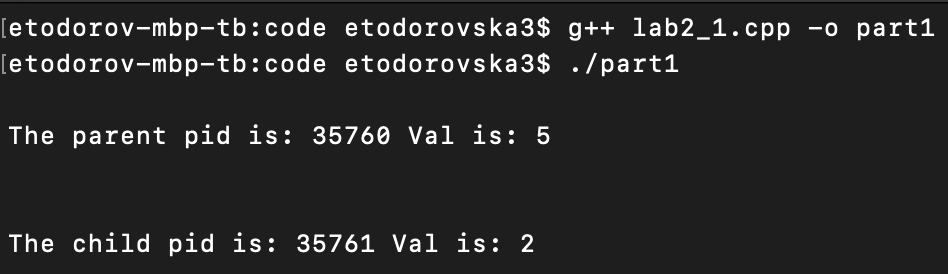
\includegraphics[width=\linewidth]{figures/Part1Output.png}
            \caption{Part 1, Console Output}
            \label{fig:part1_output}
        \end{figure}


%%%%%%%%%%%%%%%%%%%%%%%%%%%%%%%%%%%%%%%%%%%%%%%%%%%%%%%%%%%%%%%%%%%%%%%%
%%
%% Part 2
%%
%%%%%%%%%%%%%%%%%%%%%%%%%%%%%%%%%%%%%%%%%%%%%%%%%%%%%%%%%%%%%%%%%%%%%%%%

    \newpage
    \subsection{Part 2}\label{subsec:part2}
        This portion of the lab instructed us to create a program that conducts the following procedure in order:

        \begin{enumerate}
            \itemsep0em
            \item Create a new process, name: "child1"
            \item The parent (of "child1") should print its pid and wait for the termination of "child1"
            \item The "child1" process should:
            \begin{enumerate}
                \itemsep0em
                \item Call a function that subtracts two numbers passed in as arguments
                \item Print the result of that operation to console, along with the pid of the process that is printing
                \item Create a new process, name: "child2"
                \item Wait for "child2" to complete
                \item Upon completion of "child2", call a function that multiplies two numbers passed in as arguments
                \item Print the result of that operation to console, along with the pid of the process that is printing
                \item Terminate
            \end{enumerate}
            \item Meanwhile, the "child2" process should:
            \begin{enumerate}
                \itemsep0em
                \item Call a function that adds two numbers passed in as arguments
                \item Print the result of that operation to console, along with the pid of the process that is printing
                \item Terminate
            \end{enumerate}
            \item The waiting parent process should resume, and terminate
        \end{enumerate}
        Through this procedure we were allowed to either hard code the numeric arguments or read them in as user input.

        \medskip
        \noindent The source code for this portion of the lab was written and compiled on a personally owned Mac.
        The code itself is included at the end of this report in Appendix~\ref{sec:part2_source}.
        Upon implementing Part 2, compiling, and running the output to console was screenshot and is as shown on the following page in Figure \ref{fig:part2_output}.

        \begin{figure}[H]
            \centering
            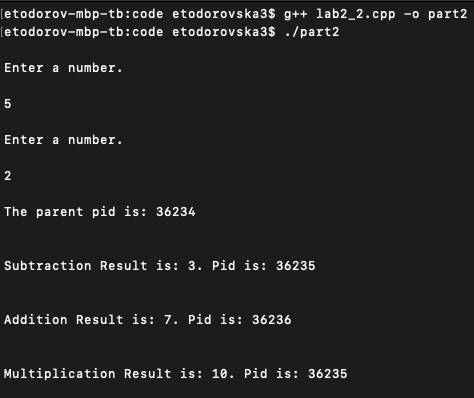
\includegraphics[width=\linewidth]{figures/Part2Output.png}
            \caption{Part 2, Console Output}
            \label{fig:part2_output}
        \end{figure}


%%%%%%%%%%%%%%%%%%%%%%%%%%%%%%%%%%%%%%%%%%%%%%%%%%%%%%%%%%%%%%%%%%%%%%%%
%%
%% Part 3
%%
%%%%%%%%%%%%%%%%%%%%%%%%%%%%%%%%%%%%%%%%%%%%%%%%%%%%%%%%%%%%%%%%%%%%%%%%

    \newpage
    \subsection{Part 3}\label{subsec:part3}
        This portion of the lab instructed us to create a program which creates \emph{n} child processes and prints their pid.
        The \emph{n} number of processes must be an even number and passed in as user input.
        If \emph{n} is not even a message should indicate that the number is odd, and terminate the program.
        The program should have one \emph{parent} process which creates \emph{n} child processes.

        \medskip
        \noindent The source code for this portion of the lab was written and compiled on a personally owned Mac.
        The code itself is included at the end of this report in Appendix~\ref{sec:part3_source}.
        Upon implementing Part 3, compiling, and running the output to console was screenshot and is as shown below.

        \begin{figure}[H]
            \centering
            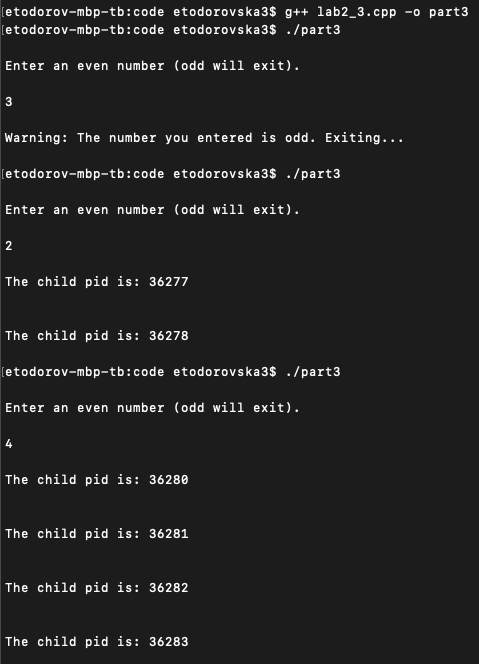
\includegraphics[width=0.75\linewidth, height=0.7\textheight]{figures/Part3Output.png}
            \caption{Part 3, Console Output}
            \label{fig:part3_output}
        \end{figure}


%%%%%%%%%%%%%%%%%%%%%%%%%%%%%%%%%%%%%%%%%%%%%%%%%%%%%%%%%%%%%%%%%%%%%%%%
%%
%% Part 4
%%
%%%%%%%%%%%%%%%%%%%%%%%%%%%%%%%%%%%%%%%%%%%%%%%%%%%%%%%%%%%%%%%%%%%%%%%%

    \newpage
    \subsection{Part 4}\label{subsec:part4}
        This portion of the lab instructed us to create a program to demonstrate the following principles:

        \begin{enumerate}
            \itemsep0em
            \item Orphan Process
            \item Zombie Process
            \item Sleeping Beauty Process
        \end{enumerate}

        \noindent The procedure also emphasized that evidence should be provided via a screenshot of the process table.
        This is provided as supplement to each principle's screenshot of console output.
        It is worth noting that each of these processes appear in the process table with different indicators.
        An "Orphan Process" will show the process dispatcher as its parent.
        A "Zombie Process" will show a "Z" in the second column of the process table.
        A "Sleeping Beauty Process" will show a "S" in the second column of the process table.

        \medskip
        \noindent The source code for this portion of the lab was written and compiled on a personally owned Mac.
        The code itself is included at the end of this report in Appendix~\ref{sec:part4_source}.
        Upon implementing Part 4, compiling, and running the output to console as well as the process table was screenshot.
        The console output is as shown below, while the process table is on the following page.

        \begin{figure}[H]
            \centering
            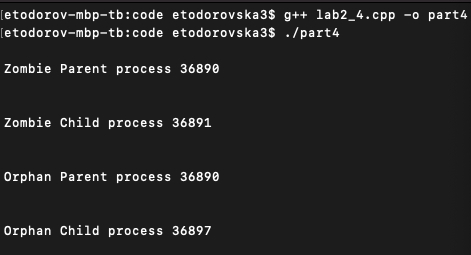
\includegraphics[width=\linewidth]{figures/Part4Output.png}
            \caption{Part 4, Console Output}
            \label{fig:part4_output}
        \end{figure}

        \begin{figure}[H]
            \centering
            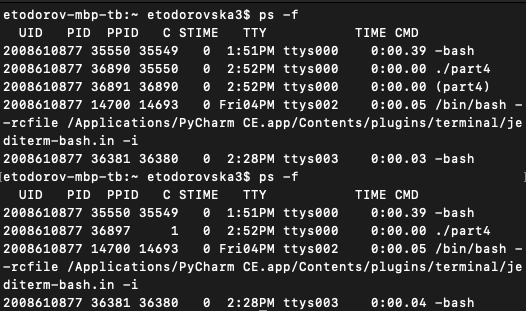
\includegraphics[width=\linewidth]{figures/Part4ProcessTable.png}
            \caption{Part 4, Process Table}
            \label{fig:part4_output}
        \end{figure}
